\documentclass[tikz,border=2pt]{standalone}
\usepackage{amsmath,amssymb}
\usepackage{pgfplots}
\pgfplotsset{compat=1.18}
\usetikzlibrary{arrows.meta,decorations.pathreplacing}
\begin{document}
% Unit whole life insurance with constant force of mortality lambda = 0.02: APV at force s is 0.02/(0.02+s).
% At delta = 0.03 it is 0.4 (first moment); at 2 delta = 0.06 it is 0.25 (second moment), not 0.4^2 = 0.16.
% Variance = 0.25 - 0.16 = 0.09.
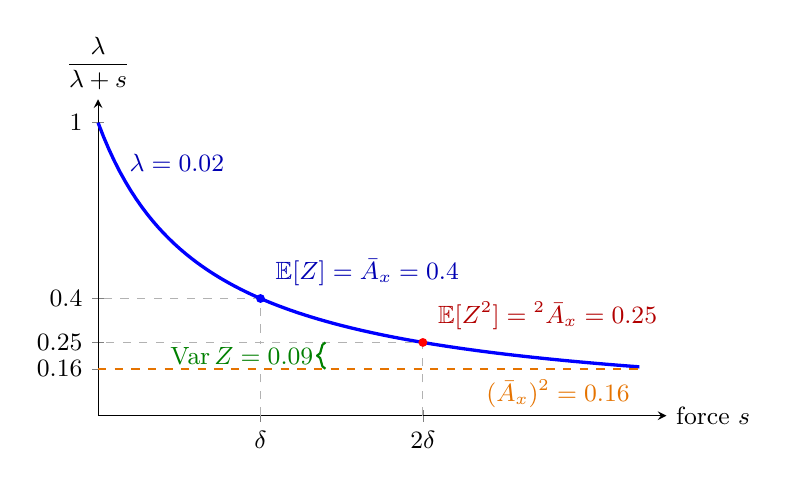
\begin{tikzpicture}[font=\small, >={Latex[length=2mm]}]
  \begin{axis}[
    axis lines=left, xmin=0, xmax=0.105, ymin=0, ymax=1.08,
    xtick={0.03,0.06}, xticklabels={$\delta$,$2\delta$},
    ytick={0.16,0.25,0.4,1}, yticklabels={$0.16$,$0.25$,$0.4$,$1$},
    xlabel={force $s$}, ylabel={$\dfrac{\lambda}{\lambda+s}$},
    xlabel style={at={(axis description cs:1,0)}, anchor=west},
    ylabel style={rotate=-90, at={(axis description cs:0,1)}, anchor=south},
    scaled x ticks=false,
    samples=100, width=8.8cm, height=5.6cm, clip=false]
    \addplot[blue, very thick, domain=0:0.1] {0.02/(0.02+x)};
    \draw[gray!60, thin, dashed] (axis cs:0.03,0) -- (axis cs:0.03,0.4) -- (axis cs:0,0.4);
    \draw[gray!60, thin, dashed] (axis cs:0.06,0) -- (axis cs:0.06,0.25) -- (axis cs:0,0.25);
    \draw[orange!90!black, thick, dashed] (axis cs:0,0.16) -- (axis cs:0.1,0.16);
    \fill[blue] (axis cs:0.03,0.4) circle (1.6pt);
    \fill[red] (axis cs:0.06,0.25) circle (1.6pt);
    \node[blue!70!black, anchor=south west] at (axis cs:0.031,0.41) {$\mathbb E[Z]=\bar A_x=0.4$};
    \node[red!70!black, anchor=south west] at (axis cs:0.061,0.26) {$\mathbb E[Z^2]={}^2\bar A_x=0.25$};
    \node[orange!90!black, anchor=north east] at (axis cs:0.1,0.155) {$(\bar A_x)^2=0.16$};
    \draw[green!50!black, thick, decorate, decoration={brace, amplitude=3pt}]
      (axis cs:0.042,0.16) -- (axis cs:0.042,0.25) node[midway, anchor=east, xshift=-3pt, fill=white, inner sep=1pt] {$\operatorname{Var}Z=0.09$};
    \node[blue!70!black, anchor=south west] at (axis cs:0.004,0.8) {$\lambda=0.02$};
  \end{axis}
\end{tikzpicture}
\end{document}
